% !TEX encoding = UTF-8
% !TEX program = lualatex

\documentclass[a4paper]{article}

\usepackage[left=1.5cm, right=1.5cm, top=1cm, bottom=2cm]{geometry}

\usepackage{mathtools, amssymb}
    \def\CC{\mathbf C}

\usepackage[no-math]{fontspec}
    \setmainfont{Noto Serif}
    \setsansfont{Noto Sans TC}
    \setmonofont{Noto Sans Mono}

\usepackage{tikz}

\begin{document}

\parindent 0pt
\parskip 1em

\newcounter{prblm}
\def\Problem{\stepcounter{prblm}[\theprblm] }

\section*{Complex Variable - Midterm Mock Exam}

\sffamily

考試時間 Test time 10:30:00 am to 12:00:00 pm; 1.5 hours.
以教室投影機時鐘為準 Using the projected clock.
用空白紙張作答 Answer on blank paper.
每題十分 Ten points per problem.
全對才給分 No partial credit.
可以帶 991 You can use fx-991 or anything weaker.
舉手問問題 Raise your hand to ask questions.

\rmfamily

\Problem Circle all the roots.
If it is a double root, circle twice, and so on.
For a pole, use squares instead of circles.
Mark the positive real line with solid lines.
Mark the negative real line with dotted lines.
(Don't answer here; draw the result on your answer sheet.)

\[ 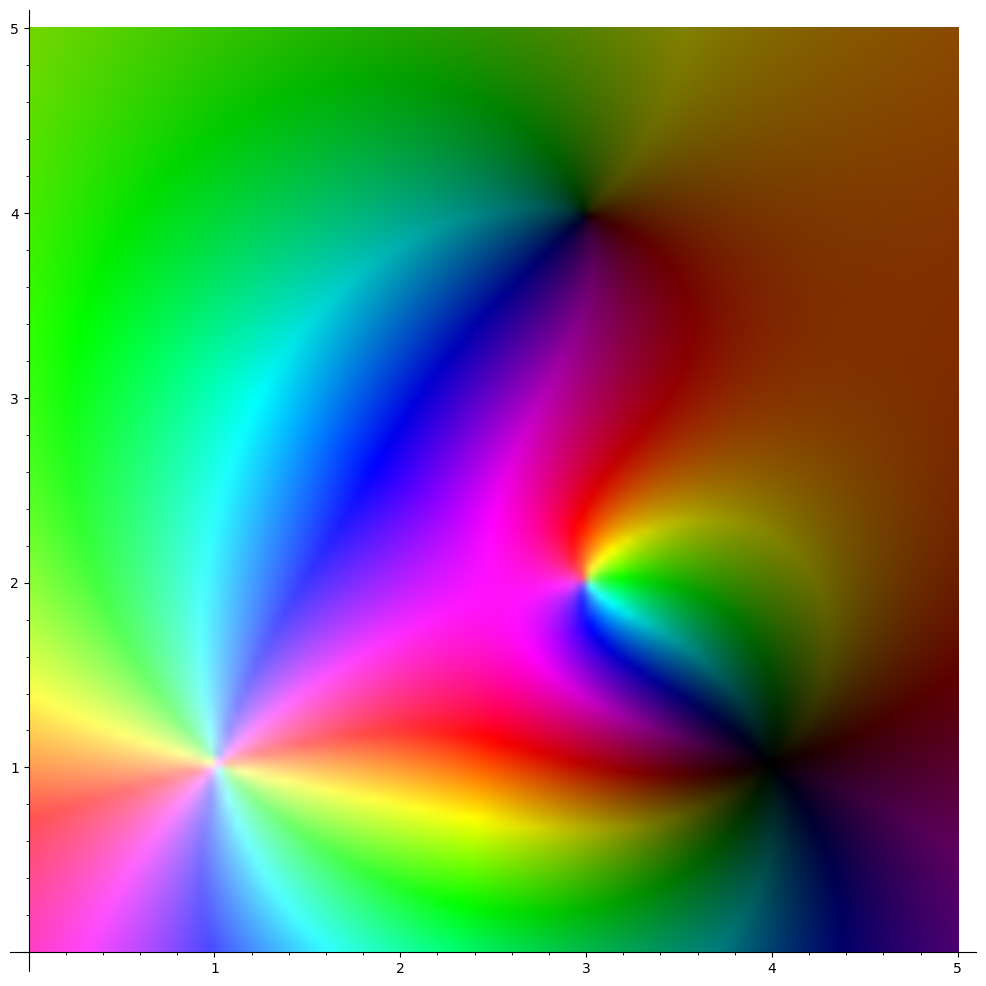
\includegraphics[height=10cm]{dc1} \]

\Problem
What maps the strip $1 < x - y < 2$ to the fan $1 < \arg z < 2$?

\Problem
Find the Taylor expansion of $\sin(\cos(z))$ at $z = 0$
up to and including the $z^6$ term.

\Problem
Assume that the Taylor expansion of $h$ exists.
Use Taylor to show that the line integral along a small square
of side length $\varepsilon$ is $O(\varepsilon^3)$.
(Don't use Green or Cauchy or so; as we are trying to ``verify'' it.)

\Problem
Let $S$ be a subset of $\CC$.
We know that, for any converging sequence of points taken from $S$,
the limit is still in $S$.
Prove that for any point in the complement of $S$,
there is an open ball around that point that does not touch $S$.

\Problem
Find (and prove) the radius of convergence of the following series
$a_n \coloneqq (10 + \exp(in))^n$.

\Problem
The Gamma function $\Gamma(z)$ is defined as
\[ \int_0^\infty t^{z-1} \exp(-t) dt \]
for all $z$ with positive real part.
Prove that $\Gamma(z + 1) = z\Gamma(z)$
for all such $z$.


\Problem
Integrate, numerically, $\exp(z^2)$
from $0$ to $\pi/2 + i$ along the straight line.
Your score is the largest number $k$ in $0 \sim 10$
such that the additive error is $< 2^{-k}$.

\Problem
Find the winding number of
$10\exp(it) + 9\exp(8it)$ for $t$ from $0$ to $2\pi$
w.r.t, $4 + 2i$.

\Problem
$x^5 - 40x^3 +3000i$
has one and only one root in the first quadrant.
Find the unit square that contains it.
Hint: start with a 16 x 16 square
and count the number of roots by integrating $f'/2\pi i f$.
If yes, cut it into four 8 x 8 smaller squares and repeat.

\end{document}